% -*- TeX-master: "main" -*-

\section{Package syntax and semantics}
\label{sec:syntax}

This section contains a definition of the syntax and semantics of the Groups package for \sbmlthreecore.  The Groups package involves four simple new object classes, \Group, \Member, \ListOfMembers and \ListOfGroups, as well as a simple extension of the existing \Model object class.  \sec{examples} contains complete examples of using the constructs in SBML models.

% --------------------------------------------------------------------------
\subsection{Namespace URI and other declarations necessary for using this package}
\label{xml-namespace}

Every SBML Level~3 package is identified uniquely by an XML namespace URI.  For an SBML document to be able to use a given Level~3 package, it must declare the use of that package by referencing its URI.  The following is the namespace URI for this version of the Groups package for \sbmlthreecore:
\begin{center}
\uri{http://www.sbml.org/sbml/level3/version1/groups/version1}
\end{center}

In addition, SBML documents using a given package must indicate whether understanding the package is required for complete mathematical interpretation of a model.  This is done using the attribute \token{required} on the \token{<sbml>} element in the SBML document.  For the Groups package, the value of this attribute must be \val{false}, because the use of the Groups package cannot change the mathematical meaning of a model.

The following fragment illustrates the beginning of a typical SBML model using \sbmlthreecore and this version of the Groups package:

\begin{example}
<?xml version="1.0" encoding="UTF-8"?>
<sbml xmlns="http://www.sbml.org/sbml/level3/version1/core" level="3" version="1"
      xmlns:groups="http://www.sbml.org/sbml/level3/version1/groups/version1"
      groups:required="false">
\end{example}


\subsection{Primitive data types}
\label{new-primitive-types}

Section~3.1 of the \sbmlthreecore specification defines a number of primitive data types and also uses a number of XML Schema 1.0 data types~\citep{biron:2000}.  We assume and use some of them in the rest of this specification, specifically \primtype{SId}, \primtype{SIdRef}, and \primtype{string}.  The Groups package also defines one more primitive type, \primtype{GroupKind}, described below.


\subsubsection{Type \fixttspace\primtypeNC{GroupKind}}
\label{primtype-groupkind}

The \primtype{GroupKind} primitive data type is used in the definition of the \Group class.  \primtype{GroupKind} is derived from type \primtype{string} and its values are restricted to being one of the following possibilities: \val{classification}, \val{partonomy}, and \val{collection}.  Attributes of type \primtype{GroupKind} cannot take on any other values.  The meaning of these three values is discussed in the context of the \Group class' definition in \sec{group-class}.


\subsection{The \class{Group} class}
\label{group-class}
\label{listofmembers-class}

The first and most central class in the Groups package is the eponymously named class \Group.  \fig{group-uml} provides the UML diagram of its definition.  The \Group class is relatively simple; it only provides an optional identifier and name, and one required attribute, \token{kind}.  These attributes and their meanings are described below.

\begin{figure}[t]
  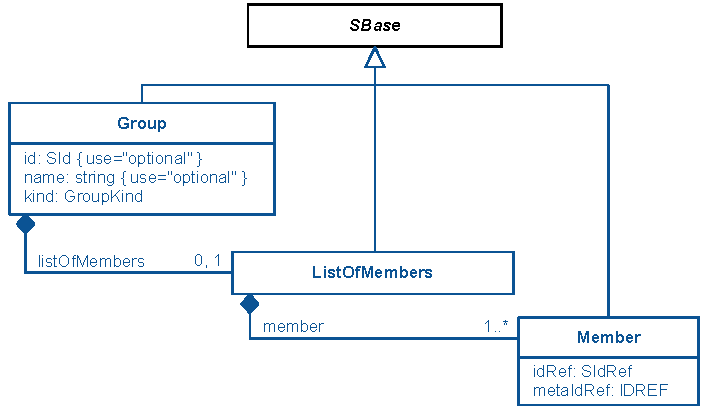
\includegraphics{figs/group-uml}
  \caption{The definition of the \Group class.  The \Member class is defined \sec{member-class}.}
  \label{group-uml}
  \label{member-uml}
\end{figure}

Since \Group is derived from \SBase, and \SBase provides the ability to attach SBO terms as well as MIRIAM annotations, the semantics of a given group in a model can be made more precise by reference to external controlled vocabularies and ontologies.  This capability is discussed further in \sec{semantics}.


\subsubsection{The \fixttspace\tokenNC{id} and \fixttspace\tokenNC{name} attributes}

The \token{id} attribute on the \Group object class serves to provide an optional handle for a group.  The attribute takes a required value of type \primtype{SId}.  The identifier of a group carries no mathematical interpretation and therefore cannot be used in mathematical formulas in a model.  The identifier can, however, be used to include a group inside another group; in other words, nested groups are permitted.

\Group also has an optional \token{name} attribute, of type \primtype{string}.  The \token{name} attribute may be used in the same manner as other \token{name} attributes on \sbmlthreecore objects; please see Section~3.3.2 of the \sbmlthreecore specification for more information.


\subsubsection{The \fixttspace\tokenNC{kind} attribute}
\label{kind-attribute}

\Group has one required attribute, \token{kind}, of type \primtype{GroupKind}.  This attribute is used to indicate the nature of the group defined by a \Group instance.  The \token{kind} attribute must always have one of the three possible values of \primtype{GroupKind}; these values have the following meanings:

\begin{description}[font=\normalfont\ttfamily\color{black},style=nextline]

\item[\token{classification}] The group represents a class, and its members have an \emph{is-a} relationship to the group.  (For example, the group could represent a type of molecule such as ATP, and the members could be species located in different compartments, thereby establishing that the species are pools of the same molecule in different locations.)

\item[\token{partonomy}] The group represents a collection of parts, and its members have a \emph{part-of} relationship to the group.  (For example, the group could represent a cellular structure, and individual compartments could be made members of the group to indicate they represent subparts of that cellular structure.)

\item[\token{collection}] The grouping is merely a collection for convenience, without an implied relationship between the members.  (For example, the group could be used to collect together multiple disparate components of a model---species, reactions, events---involved in a particular phenotype, and apply a common annotation rather than having to copy the same annotation to each component individually.)

\end{description}

\sec{semantics} and the examples in \sec{examples} further clarify the meanings of these values and the intentions behind these constructs.


\subsection{The \class{Member} class}
\label{member-class}

The \Member class is defined in \fig{member-uml}.  The class is even simpler than the \Group class, as it contains only one attribute, \token{symbol}.  The purpose of this attribute is discussed below.

Since \Member is derived from \SBase and, as mentioned above, \SBase provides both the ability to attach SBO terms as well as MIRIAM annotations, the semantics of a given member in a model can be made more precise by reference to external controlled vocabularies and ontologies.


\subsubsection{The \fixttspace\tokenNC{symbol} attribute}

The \Member class' single required attribute, \token{symbol}, has type \primtype{SIdRef}.  The value must be the identifier of an object elsewhere in the model.  An example value of \token{symbol} might be the identifier of a species in the model, or a parameter, or even another group.



\subsection{The extended \class{Model} class}
\label{model-class}
\label{extended-model-class}
\label{listofgroups-class}

The Groups package extends \sbmlthreecore's \Model class to add one list, \ListOfGroups, for holding group definitions.  \fig{extended-model-uml} provides the UML diagram for the extension.

\begin{figure}[hbt]
  \begin{overpic}{figs/group-model-uml}
    \put(85.25,12.75){\emph{\sec*{group-class}}}
  \end{overpic}
  \caption{The extensions of the \Model class.  \Group is defined in \sec{group-class}. In other respects, \Model remains defined as in the \sbmlthreecore specification.}
  \label{extended-model-uml}
\end{figure}


\subsubsection{The list of groups}

\fig{extended-model-uml} shows that the extension of \Model by the Groups package involves adding optional \token{listOfGroups} subcomponent for holding a \ListOfGroups container object.  If present, the \ListOfGroups instance must contain at least one \Group object (\sec{group-class}).  In common with other \textsf{\textbf{ListOf\rule{0.15in}{0.5pt}}} classes in SBML, \ListOfGroups is derived from \SBase.  It inherits \SBase's attributes \token{metaid} and \token{sboTerm}, as well as the subcomponents for \Annotation and \Notes, but does not add any new attributes of its own.


\section{The semantics of ``groups''}
\label{semantics}

A group \emph{G} is defined by declaring an instance of a \Group class object within the \ListOfGroups element of a \Model object. The group can be given an optional identifier (i.e., a value for its \token{id} attribute), but even if the group does not have an identifier, the act of declaring a group has the effect of creating it.

An entity \emph{X} in the model is declared to be part of group \emph{G} by listing the identifier of \emph{X} in a \Member object within the \ListOfGroups instance of \emph{G}. The following is an example to illustrate the structure:

\begin{example}
<model id="model_1"> 
  <listOfSpecies> 
    <species id="s1" .../> 
    <species id="s2" .../> 
    <species id="s3" .../> 
    <species id="s4" .../> 
  </listOfSpecies> 
  ... 
  <listOfReactions> 
    <reaction id="r1" ...> ... </reaction> 
    <reaction id="r2" ...> ... </reaction> 
  <listOfReactions> 
  ... 
  <listOfGroups xmlns="http://www.sbml.org/sbml/level3/version1/groups/version1"> 
    <group id="some_species_group" kind="collection"> 
      <listOfMembers> 
        <member symbol="s1"/> 
        <member symbol="s3"/> 
      </listOfMembers> 
    </group> 
    <group id="some_reaction_group" kind="collection"> 
      <listOfMembers> 
        <member symbol="r1"/> 
        <member symbol="r2"/> 
      </listOfMembers> 
    </group> 
  </listOfGroups> 
</model>
\end{example}

For any given group, the meaning of group membership is determined by the value of the attribute \token{kind} on the \Group object instance.  Examples of possible meanings are given in \sec{kind-attribute}.

The meaning of a group can be further refined by using annotations (either SBO terms or the \Annotation element) on the group, or the list of members. The following are the interpretations.  This possibility raises the question of how the annotations should be interpreted across the group members.  The following are the possibilities defined by the Groups package:

\begin{itemize}

\item If the annotation or SBO term is on a \Group object, it is an annotation about the group itself, not the individual members.

\item If the annotation or SBO term is on a \Member object, it is an annotation specifically about that member, and not about any other member nor the group overall.

\item If the annotation or SBO term is on \ListOfMembers, it is a short-hand that means the annotation applies to each individual member, as if the annotation were put on the individual members directly.

\end{itemize}

Finally, groups can refer to other groups, leading to the possibility of group hierarchies. To indicate a group is part of another group, one simply needs to include the first group's identifier as a member of the second group, as in the following example:

\clearpage

\begin{example}
<model id="model_2"> 
  ... 
  <listOfGroups xmlns="http://www.sbml.org/sbml/level3/version1/groups/version1"> 
    <group id="group1"> 
      <listOfMembers> 
        <member symbol="..."/> 
        <member symbol="..."/> 
      </listOfMembers> 
    </group> 
    <group id="group2"> 
      <listOfMembers> 
        <member symbol="group1"/> 
        <member symbol="..."/> 
        <member symbol="..."/> 
      </listOfMembers> 
    </group> 
  </listOfGroups> 
</model> 
\end{example}

The intended meaning of nested groups can be made more precise by annotating the group and members with appropriate MIRIAM annotations using controlled vocabulary terms that describe the meaning.


\subsection{Lack of semantic restrictions}
\label{semantic-restrictions}

The current definition of the Groups package is such that the use of Groups constructs has no impact on the mathematics of a model.  No semantic restrictions are necessary. Further, as a consequence of this, this package would not be required for proper interpretation of a model. Models could use the \token{required}=\val{false} flag on the declaration of the package on the \token{<sbml>} element in a file.

Given this lack of impact on the mathematics of a model, the Groups package cannot accomplish one aspect of SBML Level~2's \SpeciesType construct: the Groups package does not impose the restriction that two \Species objects having the same \SpeciesType cannot have the same value for their respective \token{compartment} attributes.  It is notable, however, that a properly constructed model \emph{would not place two species of the same type in the same compartment in the first place}.  Such a model would not be mathematically correct, so software tools generally take precautions to prevent this from happening when they write an SBML model.  Having a \SpeciesType component in SBML does not aid a software tool in this regard.  For the reader of a model, the prohibition against this combination in SBML Level~2 adds only a minor opportunity to do error checking.  More commonly, \SpeciesType definitions in a model are used to add type information for the reader's benefit, in the sense of indicating that certain entities are of the same kind.  However, since \SpeciesType identifiers have no mathematical meaning in Level~2, these definitions are operationally meaningless.  The only utility is to provide a type of annotation.  The Groups package provides a more flexible means of providing such annotations.

